%*******10********20********30********40********50********60********70********80

\chap{Background Theory} 
\section{Data science}
\vspace{-5mm}
It's really important to have a general idea about what "Data Science" means since this thesis procedure is strongly based on the classic Data Science Process.

We can define Data Science like a "concept to unify statistics, data analysis and their related methods" in order to understand and analyze actual phenomena with data.\cite{wiki:DataScience}\\
It includes theories drawn from many field within the broad areas of mathematics, statistics, information science and computer science.
In the computer science area are particular important the subdomains of:\\

\begin{minipage}{0.5\textwidth}
\textbf{Machine learning}: Is a subfield of computer science that gives computers the ability to learn without being explicitly programmed \cite{ArthurSamuel}. More useful specific informations about this field are provided in the following section [\ref{ML}].\\

\textbf{Cluster Analysis}: is the task of grouping a set of objects in such a way that objects in the same group (called a cluster) are more similar (in some sense or another) to each other than to those in other groups (clusters) \cite{wiki:clusterAnalysis}. \\ 


\end{minipage} \hfill
\begin{minipage}{0.50\textwidth}
\begin{figure}[H]
	\centering
    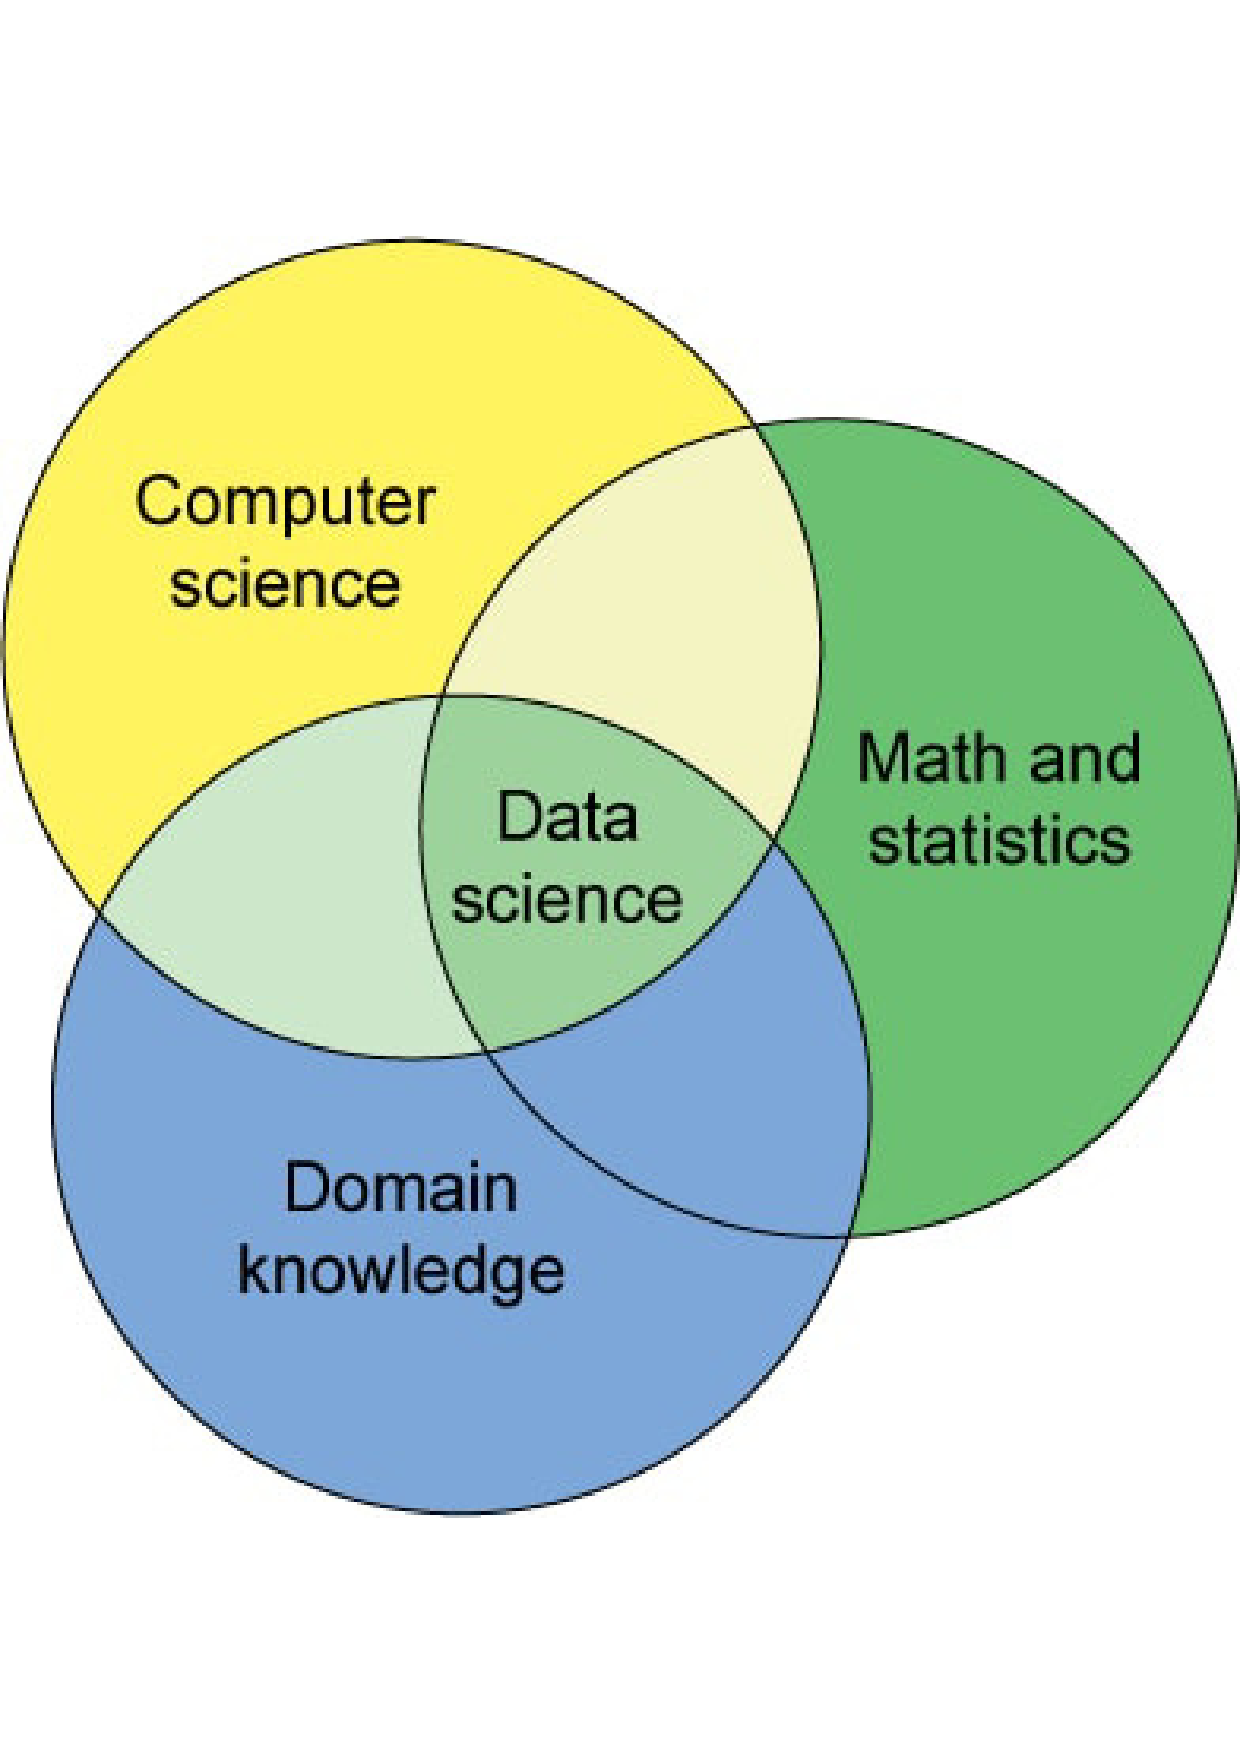
\includegraphics[trim={0 3cm 0 4cm},clip,width=0.8\textwidth]{Files/Data_Science_Concept.pdf}
    \caption{Data science concept}
    \label{fig: Data_science}
\end{figure}
\end{minipage}


\textbf{Classification}: Is the problem of identifying to which of a set of categories (sub-populations) a new observation belongs \cite{wiki:Classification}. 


\textbf{Data mining}: Is the computing process of discovering patterns in large data sets. The overall goal of the data mining process is to extract information from a data set and transform it into an understandable structure for further use. 

\textbf{Databases}: A database is an organized collection of data. It is the collection of schemas, tables, queries, reports, views, and other objects. The data are typically organized to model aspects of reality in a way that supports processes requiring information \cite{wiki:Databases}.

\textbf{Data Visualization}: It involves the creation and study of the visual representation of data. The primary goal of data visualization is to communication information clearly and efficiently via graphics and plots. \\



This study procedure is strongly based on the Data Science process designed by Joe Blitzstein and Hanspeter Pfister \cite{DataProcessFramework}, which is reported in the following image.
\begin{figure}[H]
    \centering
    \makebox[\textwidth][c]{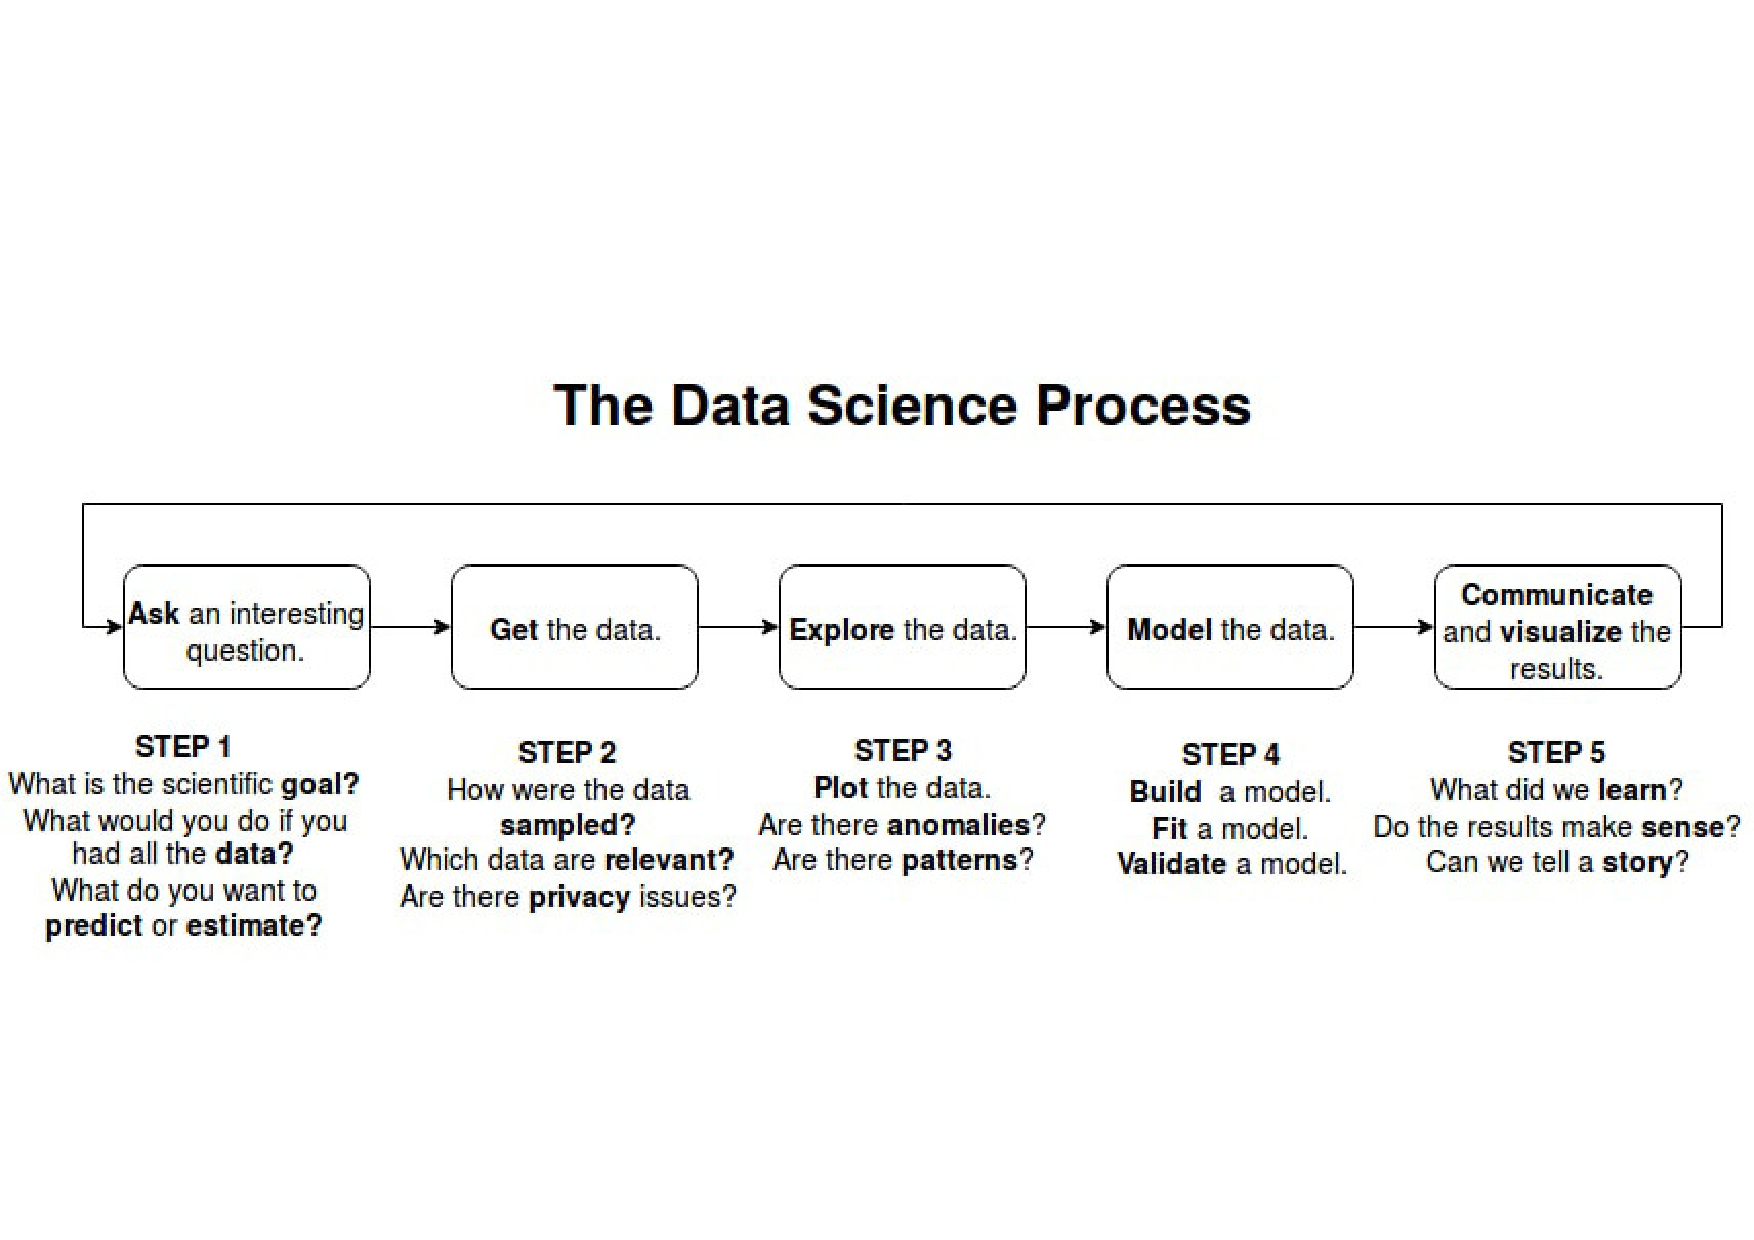
\includegraphics[trim={0 0 0 2cm},clip, width=1.2\textwidth]{Files/Data_Science_Process.pdf}}
    \caption[Data science process]{Data science process}
    \label{fig: Data_science_process}
\end{figure}

\newpage


\section{Machine learning}
\vspace{-5mm}
\label{ML}
As reported in the previous section, this subfield of computer science gives "computers the ability to learn without being explicitly programmed"\cite{ArthurSamuel}. \\
Machine learning explores the study and construction of algorithms that can learn from and make predictions on data.

There are several machine learning algorithms, each of them is used for a different purpose and a different domain \cite{wiki:ML}. For examples:

\begin{itemize}
 
  \item Artificial Neural Network: Computations are structured in terms of an interconnected group of artificial neurons. They are usually used to model complex relationships between inputs and outputs, to find patterns in data or to capture statistical structures. 
  
  \item Deep Learning: This concept consists of multiple hidden layers in an artificial neural network, and it can be successfully applied for computer vision and speech recognition.
  
  \item Clustering: Is the assignment of a set of observations into subsets, called clusters, so that observations within the same cluster are similar according to some predesignated criteria, while observations drawn from different clusters are dissimilar.
  
  \item \textbf{Regression}: Is a statistical process for estimating the relationships among variables. It includes many techniques for modeling and analyzing several variables, when the focus is on the relationship between a dependent variable and one or more independent variables. Regression analysis is widely used for prediction and forecasting, where its use has substantial overlap with the field of machine learning. This specific domain contains the model used in this study \cite{wiki:Regression}.
  
 \end{itemize}  

\newpage

\subsection{Time Series analysis and predictions}
  \vspace{-5mm}
Time Series forecasting is an important area of machine learning, but that is often neglected. Is that important mainly beause there are so many prediction problems that involve a time component, and these problems are neglected because it is this time component that makes time series problems more difficult to handle \cite{previousWork}.

" A time series is a sequence of observations taken sequentially in time \cite{TimeSeries}. " 

Classic example of a time series dataset:

\begin{tabular}{ | l | l | }
\hline 		\textbf{Date}	&	\textbf{Paramater} \\ \hline
				Time \#1	&	observation \\ \hline	
				Time \#2	&	observation \\ \hline	
				Time \#3	&	observation \\ \hline											
\end{tabular}

Understanding a dataset is called "time series analysis" and it can helps to make better prediction, but sometimes it's not required and can results a large investment in time and technical expertise.

Making predictions could be called "time series forecasting" and it involves taking models fit on historical data and using them to predict future observations.

\subsection{Autoregressive integrated moving average (ARIMA)}
\vspace{-5mm}
A widely used statistical method for time series forecasting is the ARIMA model. Since this a very complicated and deep topic, this study provided just an initial implementation and description of it. During this section are provided some basic definitions and overviews enough to understand the general logic behind a forecasting system. If you are particularly interested in this topic my suggestion is to read more about it.

\textbf{AR model}: an autoregressive model is a representation of a type of random process; as such, it is used to describe certain time-varying processes in nature, economics, etc. The autoregressive model specifies that the output variable depends linearly on its own previous values and on a stochastic term (an imperfectly predictable term); thus the model is in the form of a stochastic difference equation.\cite{wiki:AR}

\textbf{MA model}: a moving-average model is a common approach for modeling univariate time series. The moving-average model specifies that the output variable depends linearly on the current and various past values of a stochastic (imperfectly predictable) term.\cite{wiki:MA}

\newpage

\textbf{ARMA model}: an autoregressive-moving-average model provides a parsimonious description of a stationary stochastic process in terms of two polynomials, one for the autoregression and the second for the moving average. Basically it combines both AR and MA models into a unique representation.\cite{wiki:ARMA}

\textbf{ARIMA model}: is a generalization of an autoregressive moving average (ARMA) model. Both of these models are fitted to time series data either to better understand the data or to predict future points in the series (forecasting).\\
This model is applied in some cases where data show evidence of non-stationarity, where an initial differencing step (corresponding to the "integrated" part of the model) can be applied one or more times to eliminate the non-stationarity.\cite{wiki:ARIMA}

\textbf{ARIMA(p, d, q)}
  \vspace{-5mm}
\begin{itemize}
 \setlength{\itemsep}{-5pt}
\item \textbf{p} is the number of autoregressive terms (How many preceding values are examinated for the current value’s forecast).

\item \textbf{d} is the number of nonseasonal differences needed for stationarity.

\item \textbf{q} is the number of lagged forecast errors in the prediction equation. 
\end{itemize}

\newpage

\section{Aquaculture in Norway}
\vspace{-5mm}
During the last years there has been a very rapid development of Norway's aquaculture industry, and the production of Atlantic salmon has grown to become a major sector of its economy. The industry is now an economic pillar for several Norwegian coastal communities.\cite{SenCanada}

The Aquaculture industry in Norway is dominated by its finfish\footnote{A bony fish, such as a salmon, or a cartilaginous fish, such as a shark, especially in contrast to a shellfish or other aquatic animal.} sector, with Atlantic salmon and Rainbow trout accounting for 93.9\% and 5.8\% respectively of total volume produced.

This business takes place in the counties along most of the country's coastline. In the finfish sector Nordland is the dominant producer county, with Hordaland coming second, Møre og Romsdal third, and Troms fourth.

\begin{figure}[h]
    \makebox[\textwidth][c]{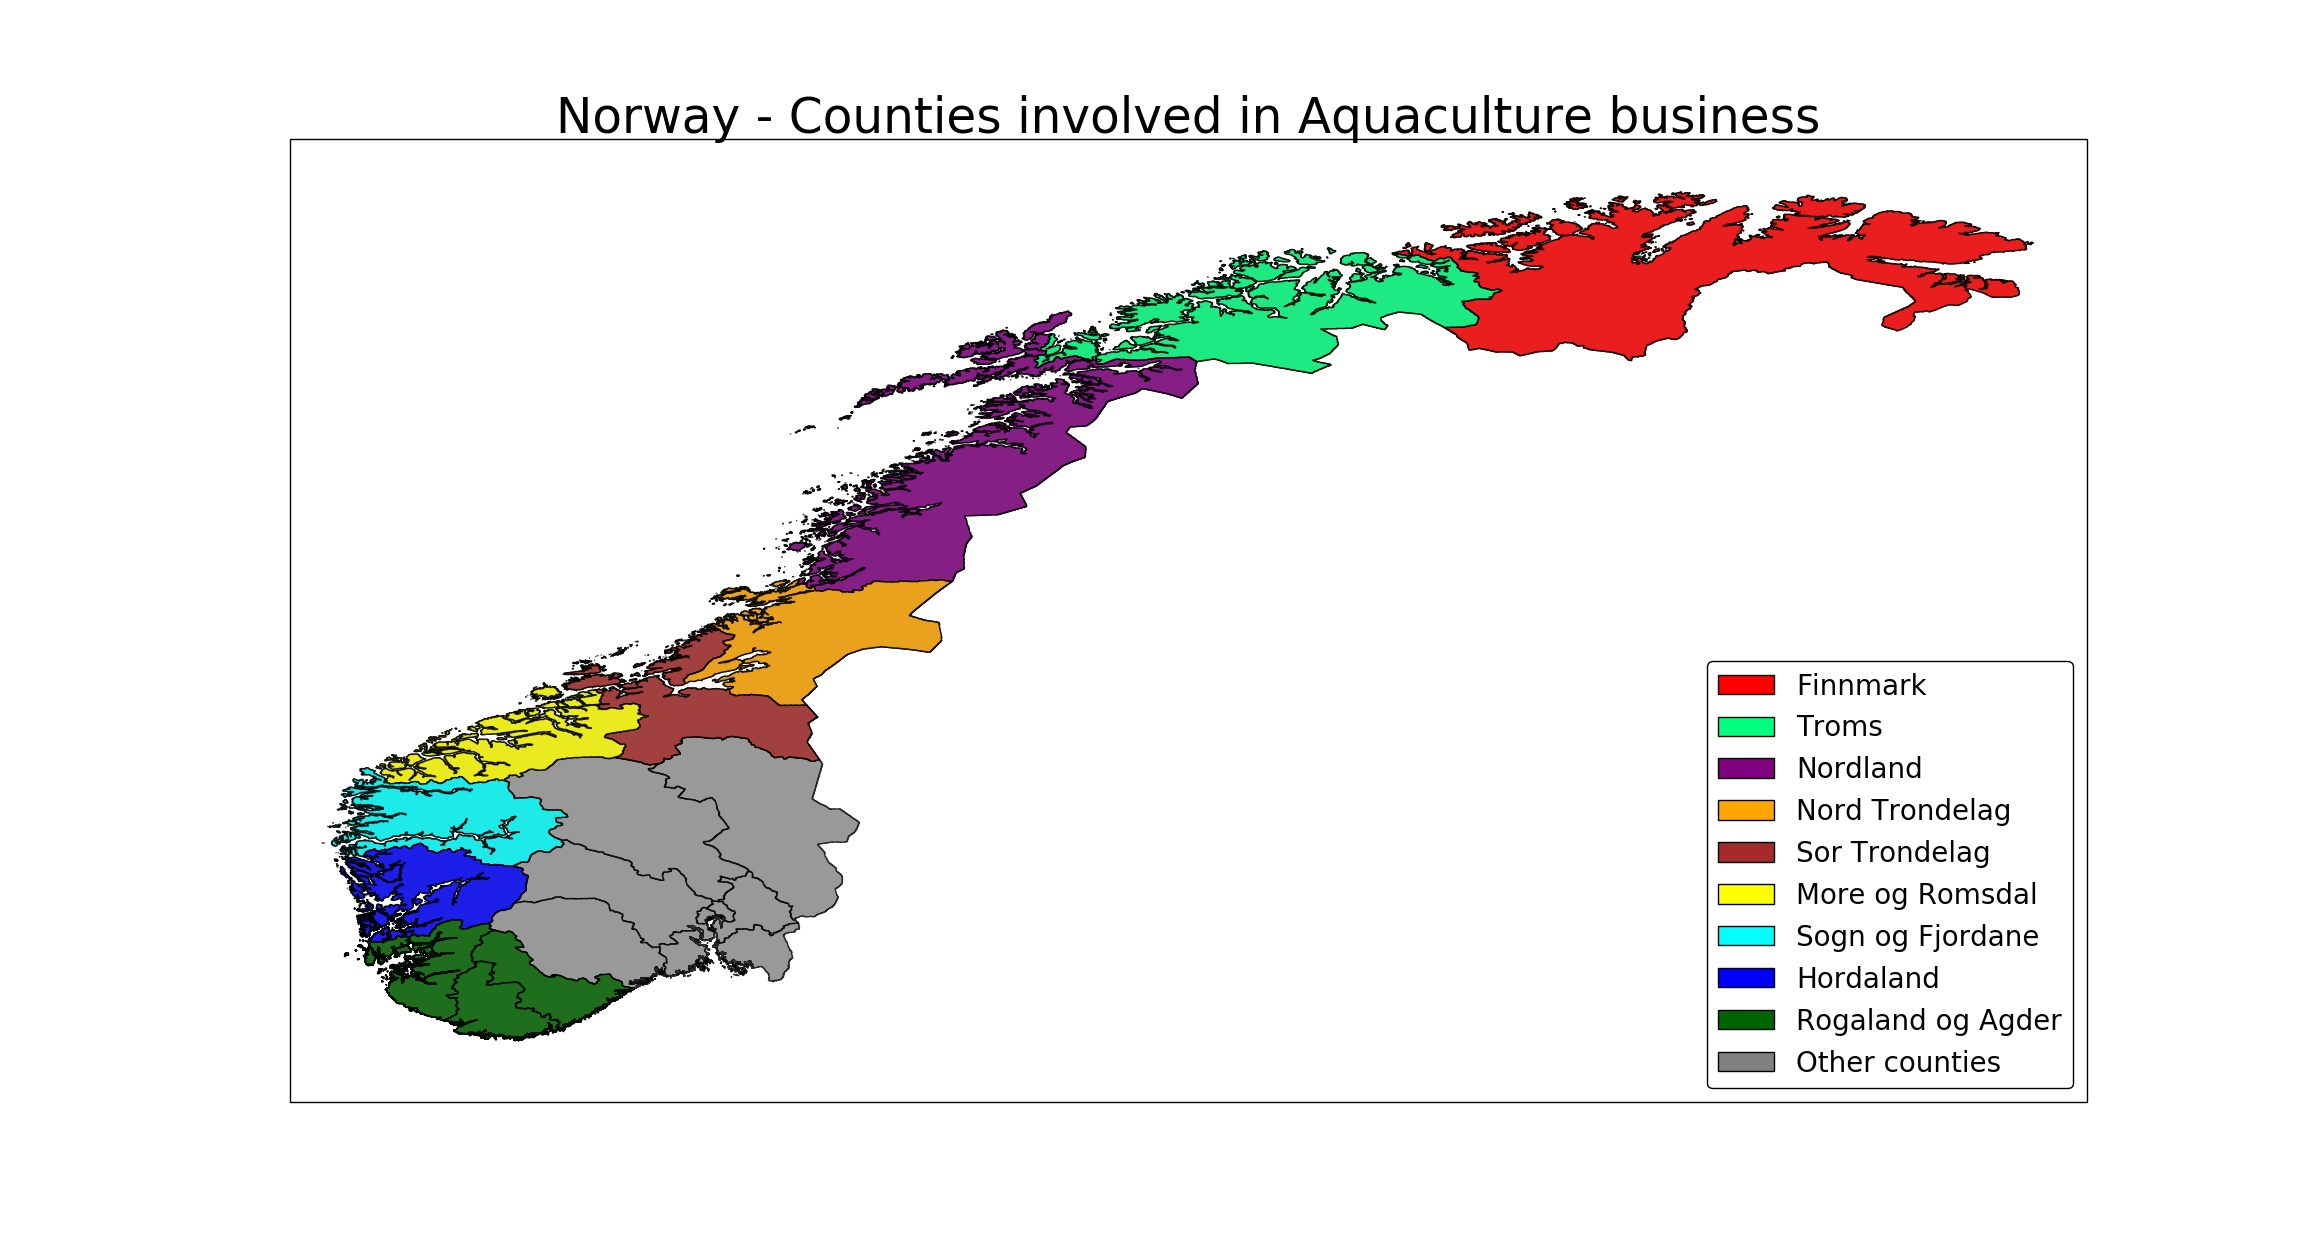
\includegraphics[width=1.2\textwidth, trim={0 0 0 0cm},clip,]{Files/Counties.pdf}}
    \caption[Norwegian counties involved in aquaculture business]{Norwegian counties involved in aquaculture business}
    \label{fig: Norway_Counties}
\end{figure}